\chapter{The ARM Cortex-M0}

At the core of a microcontroller is the CPU. Our CPU is called the Cortex-M0 and is designed by Advanced RISC Machines (ARM).
The ARM Cortex-M0 CPU is certainly the most interesting block inside the STM32F051C6. This is where all processing happens, hence this is where the instructions which we write will run. It is therefore essential that we have an intricate understanding of the CPU so that we may write useful code for it. This chapter seeks to explore the CPU in some detail.

\section{Programmer's Model of the CPU}
\begin{figure}[t]
  \centering
  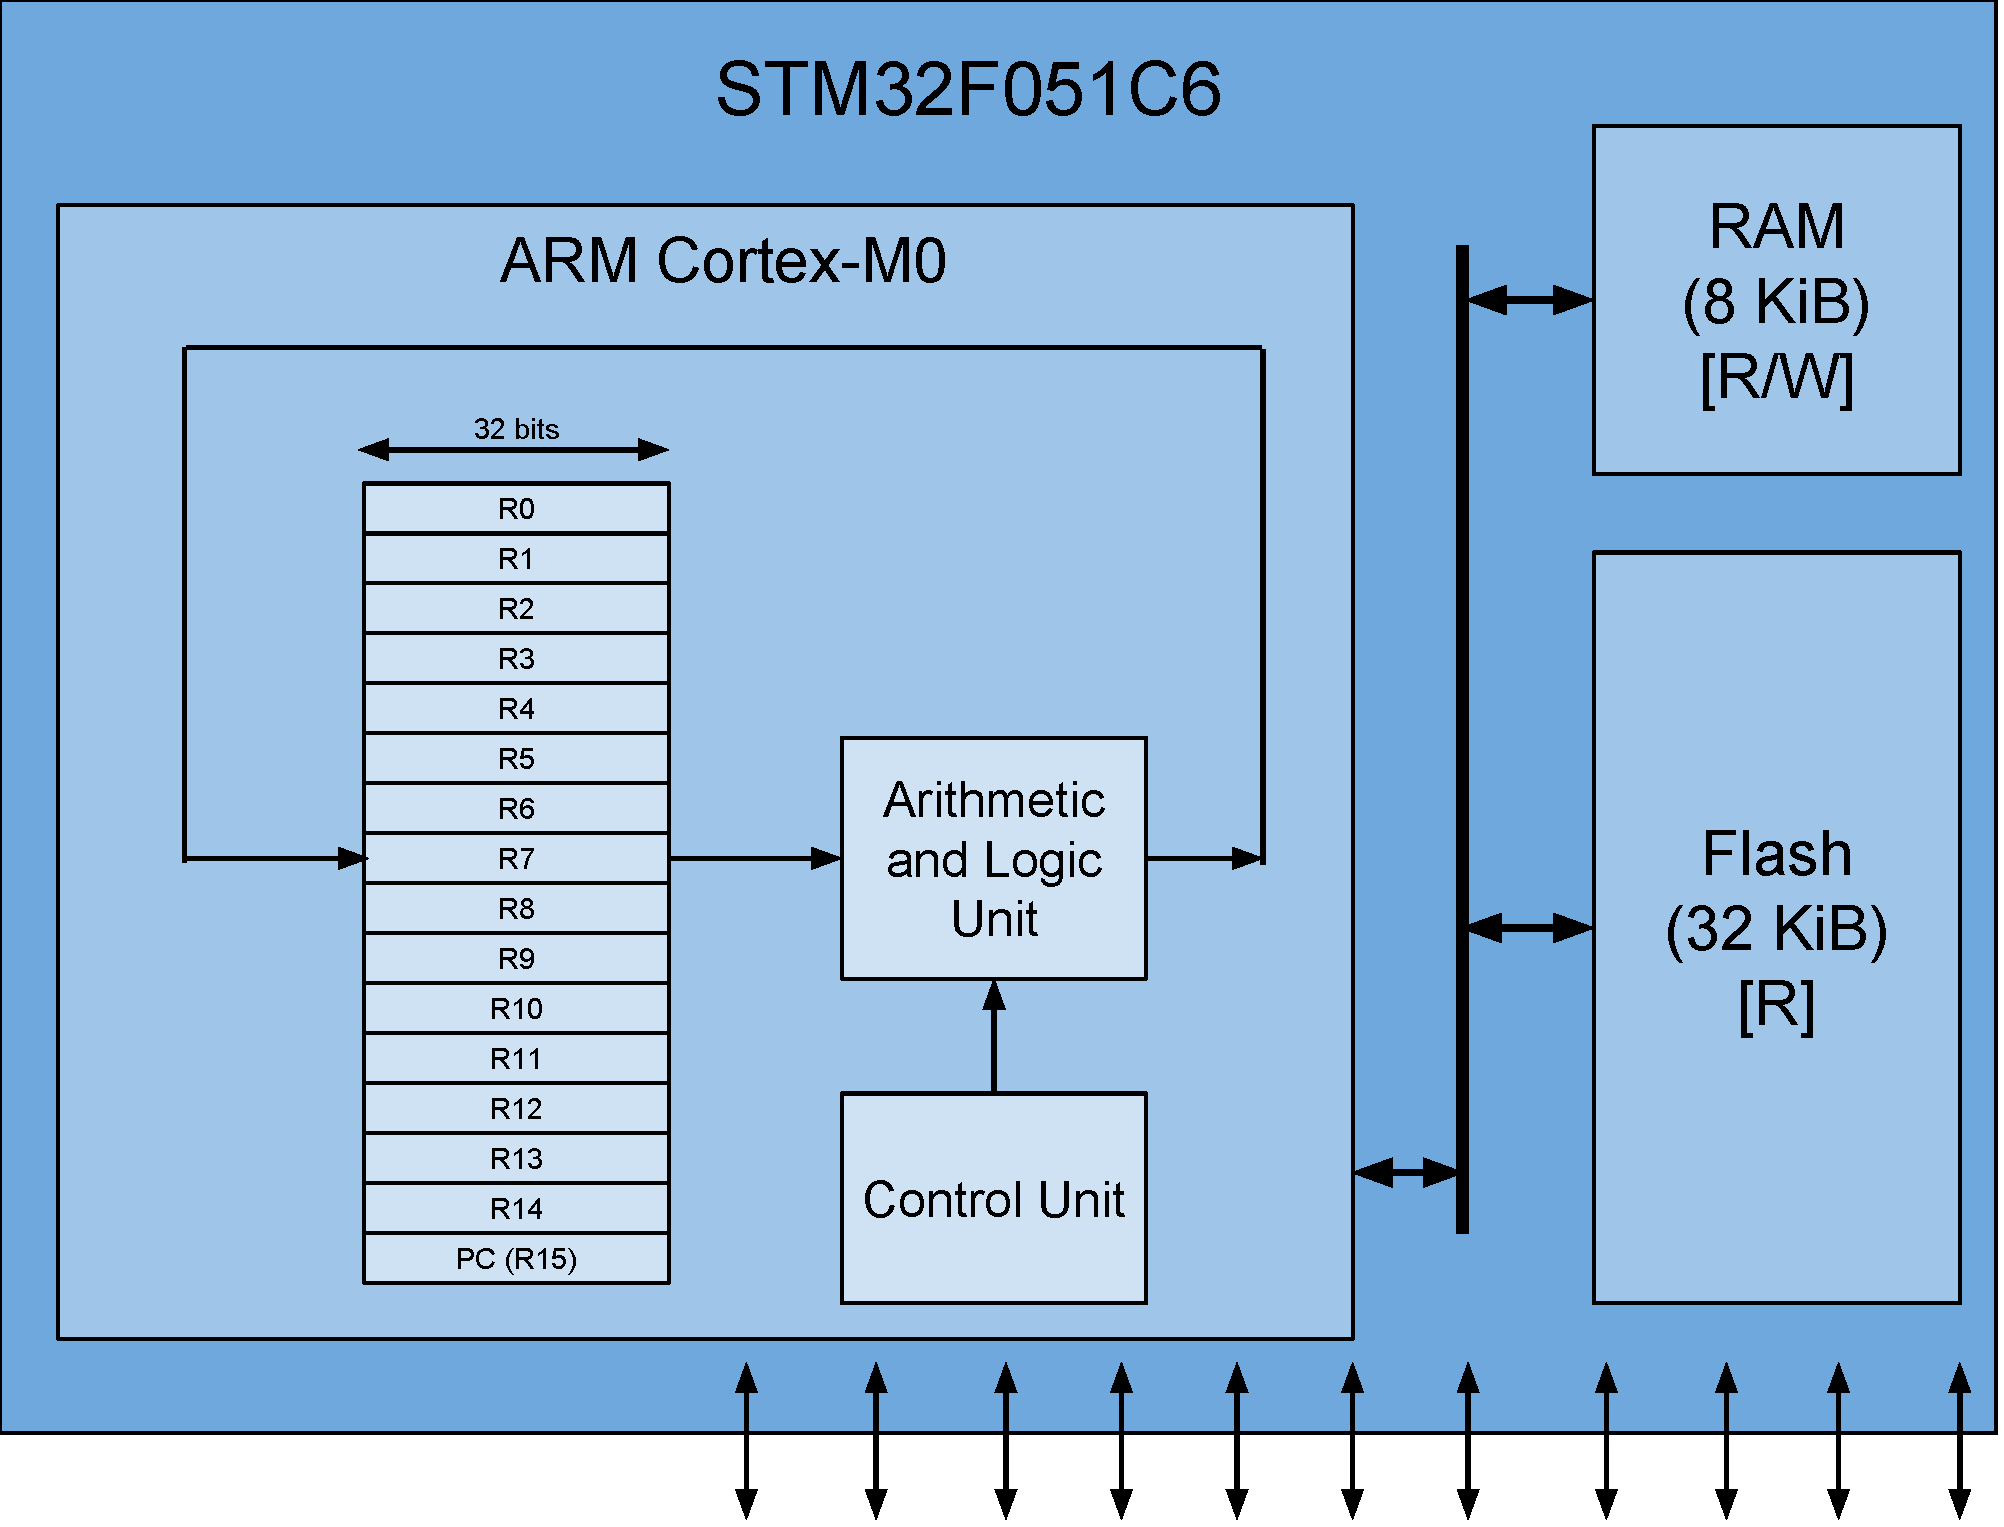
\includegraphics[width=0.9\textwidth]{./fig/programmers_model_v1.pdf}
  \caption{A view of the internals of the STM32F051 with the ARM Cortex-M0 expanded}
  \label{fig:prog_mod_v1}
\end{figure}
A programmer's model is a representation of the inner workings of the CPU with sufficient detail to allows us to develop code for the CPU, but no unnecessary detail. The expanded view of the CPU which will now be discussed can be seen in \autoref{fig:prog_mod_v1}. This simple model of a CPU is a set of CPU registers, an Arithmetic and Logic Unit (ALU) and a control Unit. The CPU registers are blocks of storage each 32 bits wide which the CPU has the ability to operate on. Only data which is inside a CPU register can be operated on by the CPU. The ARM Cortex-M0 has 16 such registers. 

The ALU is that which performs the operations on the registers. It can take data from registers as inputs, do very basic processing and store the result in CPU registers. 

The control unit manages execution by telling the ALU what to do. Together, the registers, ALU and control are able to execute instructions. 
Examples of instructions which the CPU is able to execute:
\begin{enumerate}
  \item adding the contents of R0 and R1 and storing the result in R6
  \item copying the contents of R3 into R0
  \item doing a logical XOR of the contents of R3 with the contents of R4 and storing the result in R3
  \item moving the number 42 into R5
\end{enumerate}


\section{CPU Architecture}
This section will explore some CPU architectures and compare them to the architecture of the Cortex-M0.

The Cortex-M0 makes use of a Von Neumann architecture. This means that there is a single bus which connects all of the parts (such as CPU, RAM, flash)  inside the microcontroller. The implication of this is that the CPU cannot fetch an instruction from flash at the same time as it moves data in or out of RAM. This limitation allows for a much simpler architecture, but at the expense of performance. 

Other microcontrollers (even others in the Cortex-M series like the Cortex-M3) follow a Harvard architecture, meaning that there are separate buses used for fetching instructions and moving data around. This allows faster execution as instructions can be fetched at the same time as data is loaded or stored. However, it necessitates greater complexity and more transistors. \\

It's been said that the ARM Cortex-M0 is a 32-bit processor. For comparison, the processor which we used in this course previously (MC9S08GT16A) was an 8-bit processor. Your personal computer probably has a 64-bit CPU. 16-bit CPUs also used to be quite common. So what exactly does it mean when we say that the processor is 32-bits? Essentially, the number of bits which a processor is said to be referrers to the size of the data bus. In other words: the amount of data which the processor is able to move around internally or perform arithmetic and logic operations on. Hence, with a 32-bit processor, we can move 32 bits of data from one spot in memory to another in just once instruction or add two 32-bit numbers in a single instruction. If you had a 8-bit processor, it would cost 4 instructions to interact with 32 bits of data.

\section{Program Counter}
The Program Counter is a special register in the CPU, specifically: R15. It's called "special" because it has a specific, fixed purpose and cannot be used as a general purpose register like the other registers can. It's purpose is keeping track of were we are in the execution of a program. All instructions which need to be executed are laid out sequentially in flash, each instruction occupying a halfword of memory. Hence, each instruction has a defined address. The PC points to (ie: hold the address of) the instruction which is about to be fetched from flash to be executed. 

Typically, the value of the PC is simply incremented by 2 in order to cause it to point to the next instruction in memory. Why 2? Each instruction is 16 bits wide, so occupies 2 memory addresses. Hence the difference in \emph{addresses} from instruction n to instruction n+1 is 2. However, it's possible to alter the flow of execution of a program by issuing a \emph{branch} instruction which will cause the PC to be incremented or decremented by a different amount. Branches will be explored later.

\subsection{Three stage pipeline}
There is a bit more complexity to the program counter than initially apparent. It's worth understanding this extra intricacy as it affects how other instructions which depend on the program counter work. 
The ARM Cortex-M0 implements a three stage pipeline. This means that an instruction is broken up into three parts, and executed over the course of three clock cycles. The parts are:
\begin{itemize}
  \item \textbf{fetch:} the instruction which the program counter points to is pulled into the CPU.
  \item \textbf{decode:} the CPU control unit "looks" at the 16 bits which represent the instruction, and figures out what action it must take.
  \item \textbf{execute:} the CPU runs the instruction, causing data to be modified.
\end{itemize}
The fact that the CPU is pipelined means that different instructions can be going through different phases \emph{at the same time}. In other words, one instruction can be being fetched while another is being decoded while another is being executed. 
As an example, assume we have three instructions which we want to execute, instruction A, instruction B and instruction C. The three instructions being run through the pipeline is shown graphically in \autoref{fig:pipeline}. It's critical to note how the program counter is always pointing to the instruction being \emph{fetched}. This makes sense as the job of the program counter after all is to facilitate keeping track of which instruction must be fetched. For this reason, when an instruction is being executed, the PC is actually pointing to two instructions (four bytes) further ahead in memory, and \emph{not} at the address of the instruction in execution. Hence, when an instruction in execution uses the PC, the value which will be used is the address of the instruction plus four.
\begin{figure}
  \centering
  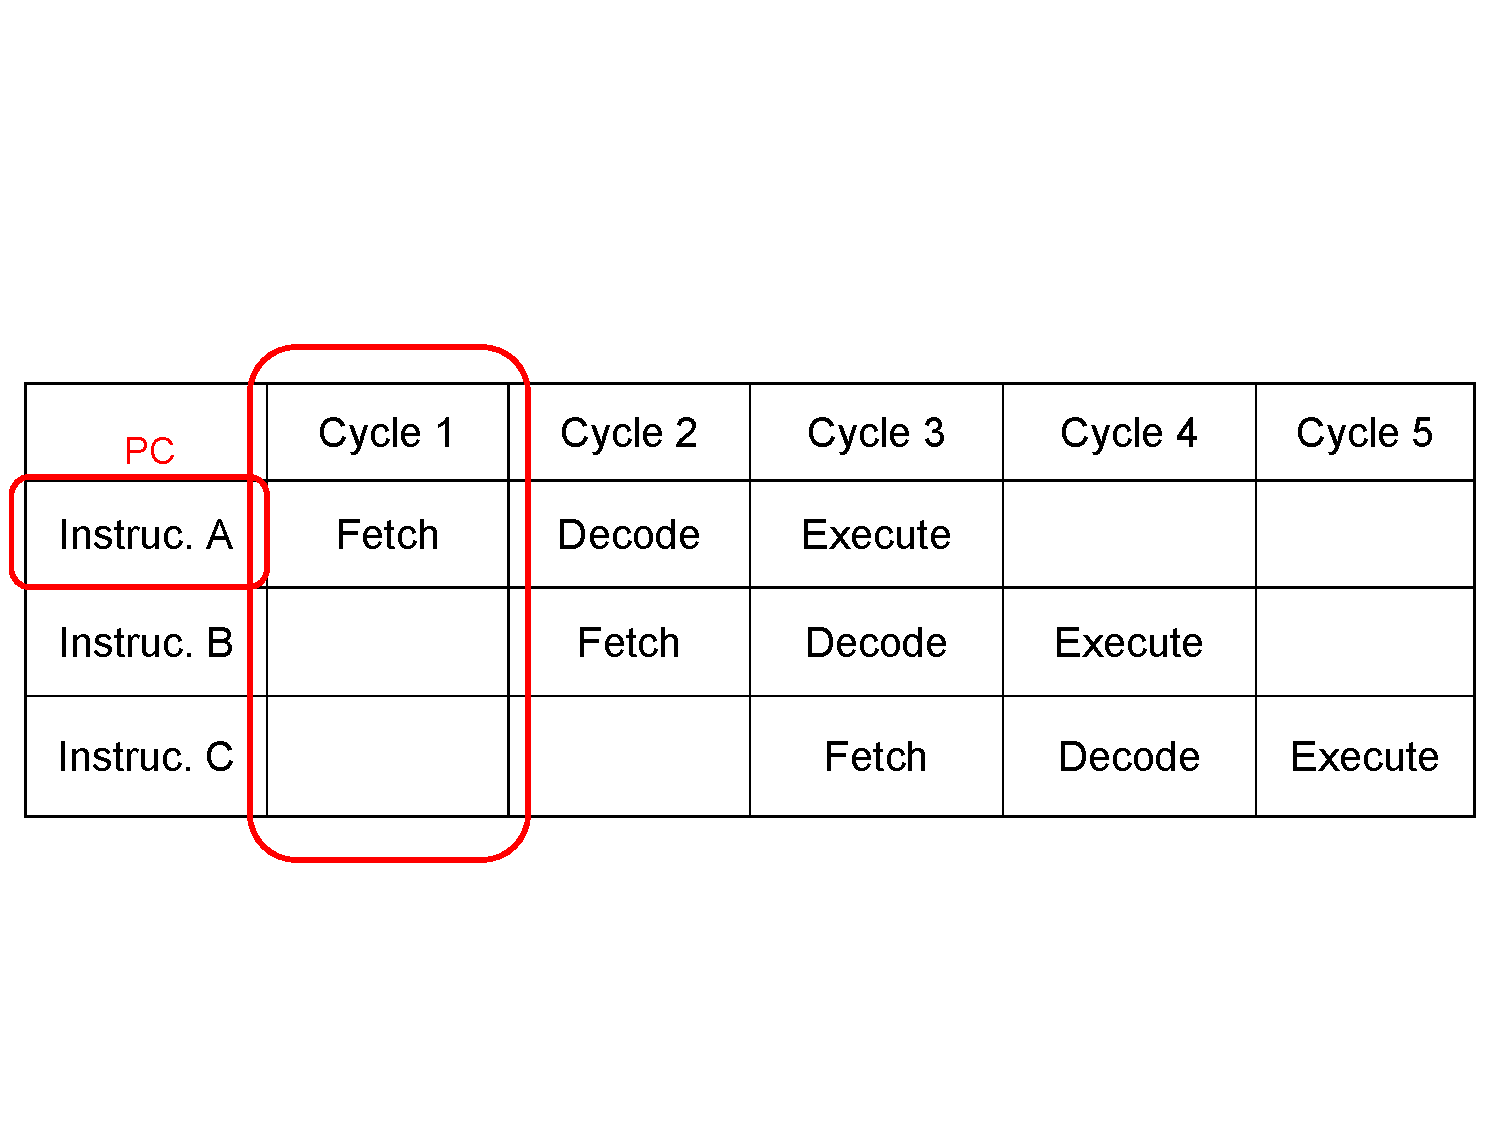
\includegraphics[page=1, clip=true, trim=1mm 40mm 1mm 57mm, width=0.8\textwidth]{./fig/pipeline.pdf}
  \includegraphics[page=2, clip=true, trim=1mm 40mm 1mm 57mm, width=0.8\textwidth]{./fig/pipeline.pdf}
  \includegraphics[page=3, clip=true, trim=1mm 40mm 1mm 57mm, width=0.8\textwidth]{./fig/pipeline.pdf}
\caption{Showing three instructions being run through a three stage pipeline, as well as where the PC is pointing every cycle}
\label{fig:pipeline}
\end{figure}

\section{Reset Vector}
When the CPU starts up, where should it begin execution from? It could have a fixed location, perhaps the first address in flash which is defined to hold the first instruction to execute. This however would limit out flexibility. Very often we want other data to come before out instructions. Exactly what this other data is will be explored in more detail later, but suffice to say that it's useful to have flexibility to define where the first instruction is located. This is done with the reset vector. When it boots up, the CPU fetches number which it must initialise the PC to from the address 0x0800 0004. This address is known as the reset vector as it points to the first instruction to be executed after reset.
